%%%%%%%%%%%%%%%%%%%%%%%%%%%%%%%%%%%%%%%%%%%%%%%%%%%%%%%%%%%%%%%%%%%%
%% I, the copyright holder of this work, release this work into the
%% public domain. This applies worldwide. In some countries this may
%% not be legally possible; if so: I grant anyone the right to use
%% this work for any purpose, without any conditions, unless such
%% conditions are required by law.
%%%%%%%%%%%%%%%%%%%%%%%%%%%%%%%%%%%%%%%%%%%%%%%%%%%%%%%%%%%%%%%%%%%%

\documentclass{beamer}
\usetheme[faculty=science, university=uu, logo=uu-logo]{fibeamer}
\usepackage[utf8]{inputenc}
\usepackage[
  main=english %% By using `czech` or `slovak` as the main locale
                %% instead of `english`, you can typeset the
                %% presentation in either Czech or Slovak,
                %% respectively.
                %% The additional keys allow foreign texts to be
]{babel}        %% typeset as follows:
%%
%%   \begin{otherlanguage}{czech}   ... \end{otherlanguage}
%%   \begin{otherlanguage}{slovak}  ... \end{otherlanguage}
%%
%% These macros specify information about the presentation
\title{VLITE-Fast} %% that will be typeset on the
\subtitle{VLA's P-band commensal search engine} %% title page.
\author{Suryarao Bethapudi}
%% These additional packages are used within the document:
\usepackage{ragged2e}  % `\justifying` text
\usepackage{booktabs}  % Tables
\usepackage{tabularx}
\usepackage{tikz}      % Diagrams
\usetikzlibrary{calc, shapes, backgrounds}
\usepackage{amsmath, amssymb}
\usepackage{url}       % `\url`s
\usepackage{listings}  % Code listings
\frenchspacing
%% add image path
\graphicspath{{figures/}}
\begin{document}
\frame{\maketitle}

\AtBeginSection[]{% Print an outline at the beginning of sections
\begin{frame}<beamer>
	\tableofcontents[currentsection]
\end{frame}}

%%%%%%%%%% MATTER

\section{Fast Radio Bursts}
%% matter tex
%% begins with section

\begin{frame}
\begin{center}
\vspace*{\vfill}
{\Large F}ast \hfill $\sim$ milli-second
{\Large R}adio \hfill $\sim$ radio-regime \emph{???}
{\Large B}urst \hfill $\sim$ Like an explosion
\begin{figure}
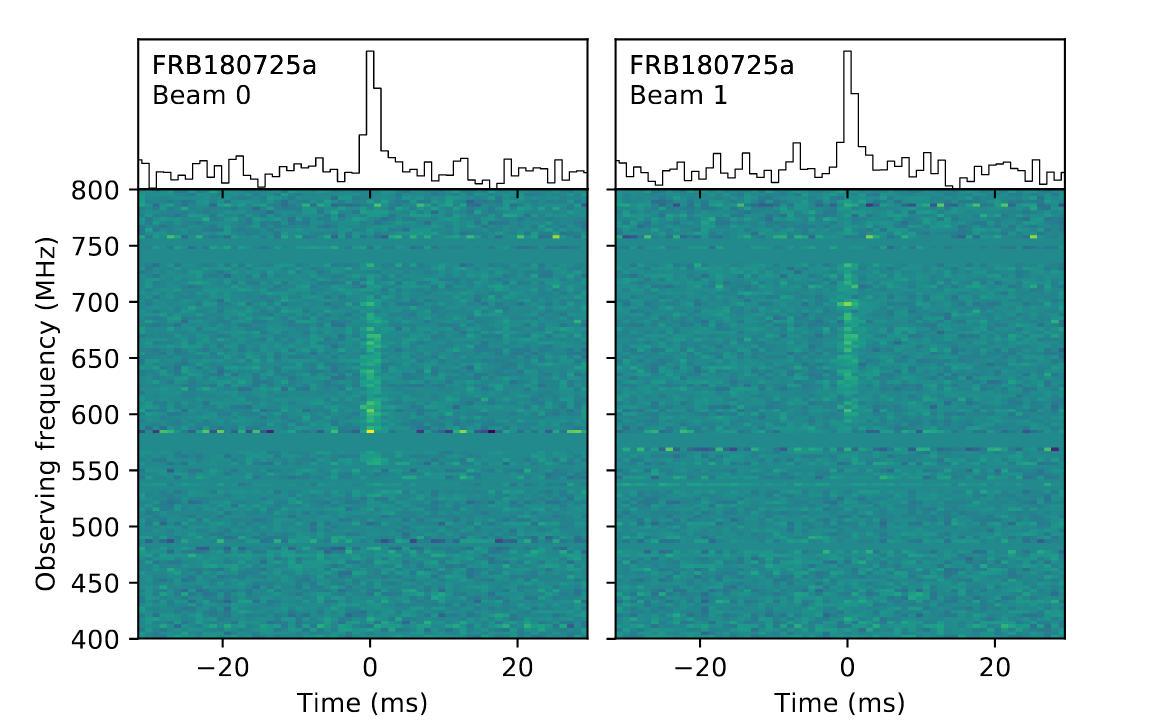
\includegraphics[width=\textwidth, keepaspectratio]{frbdef.png}
\caption{ATel#11901:First CHIME/FRB detection at 400-800 MHz}
\end{figure}
\vspace*{\vfill}
\end{center}
\end{frame}

\begin{frame}
\begin{figure}
\centering
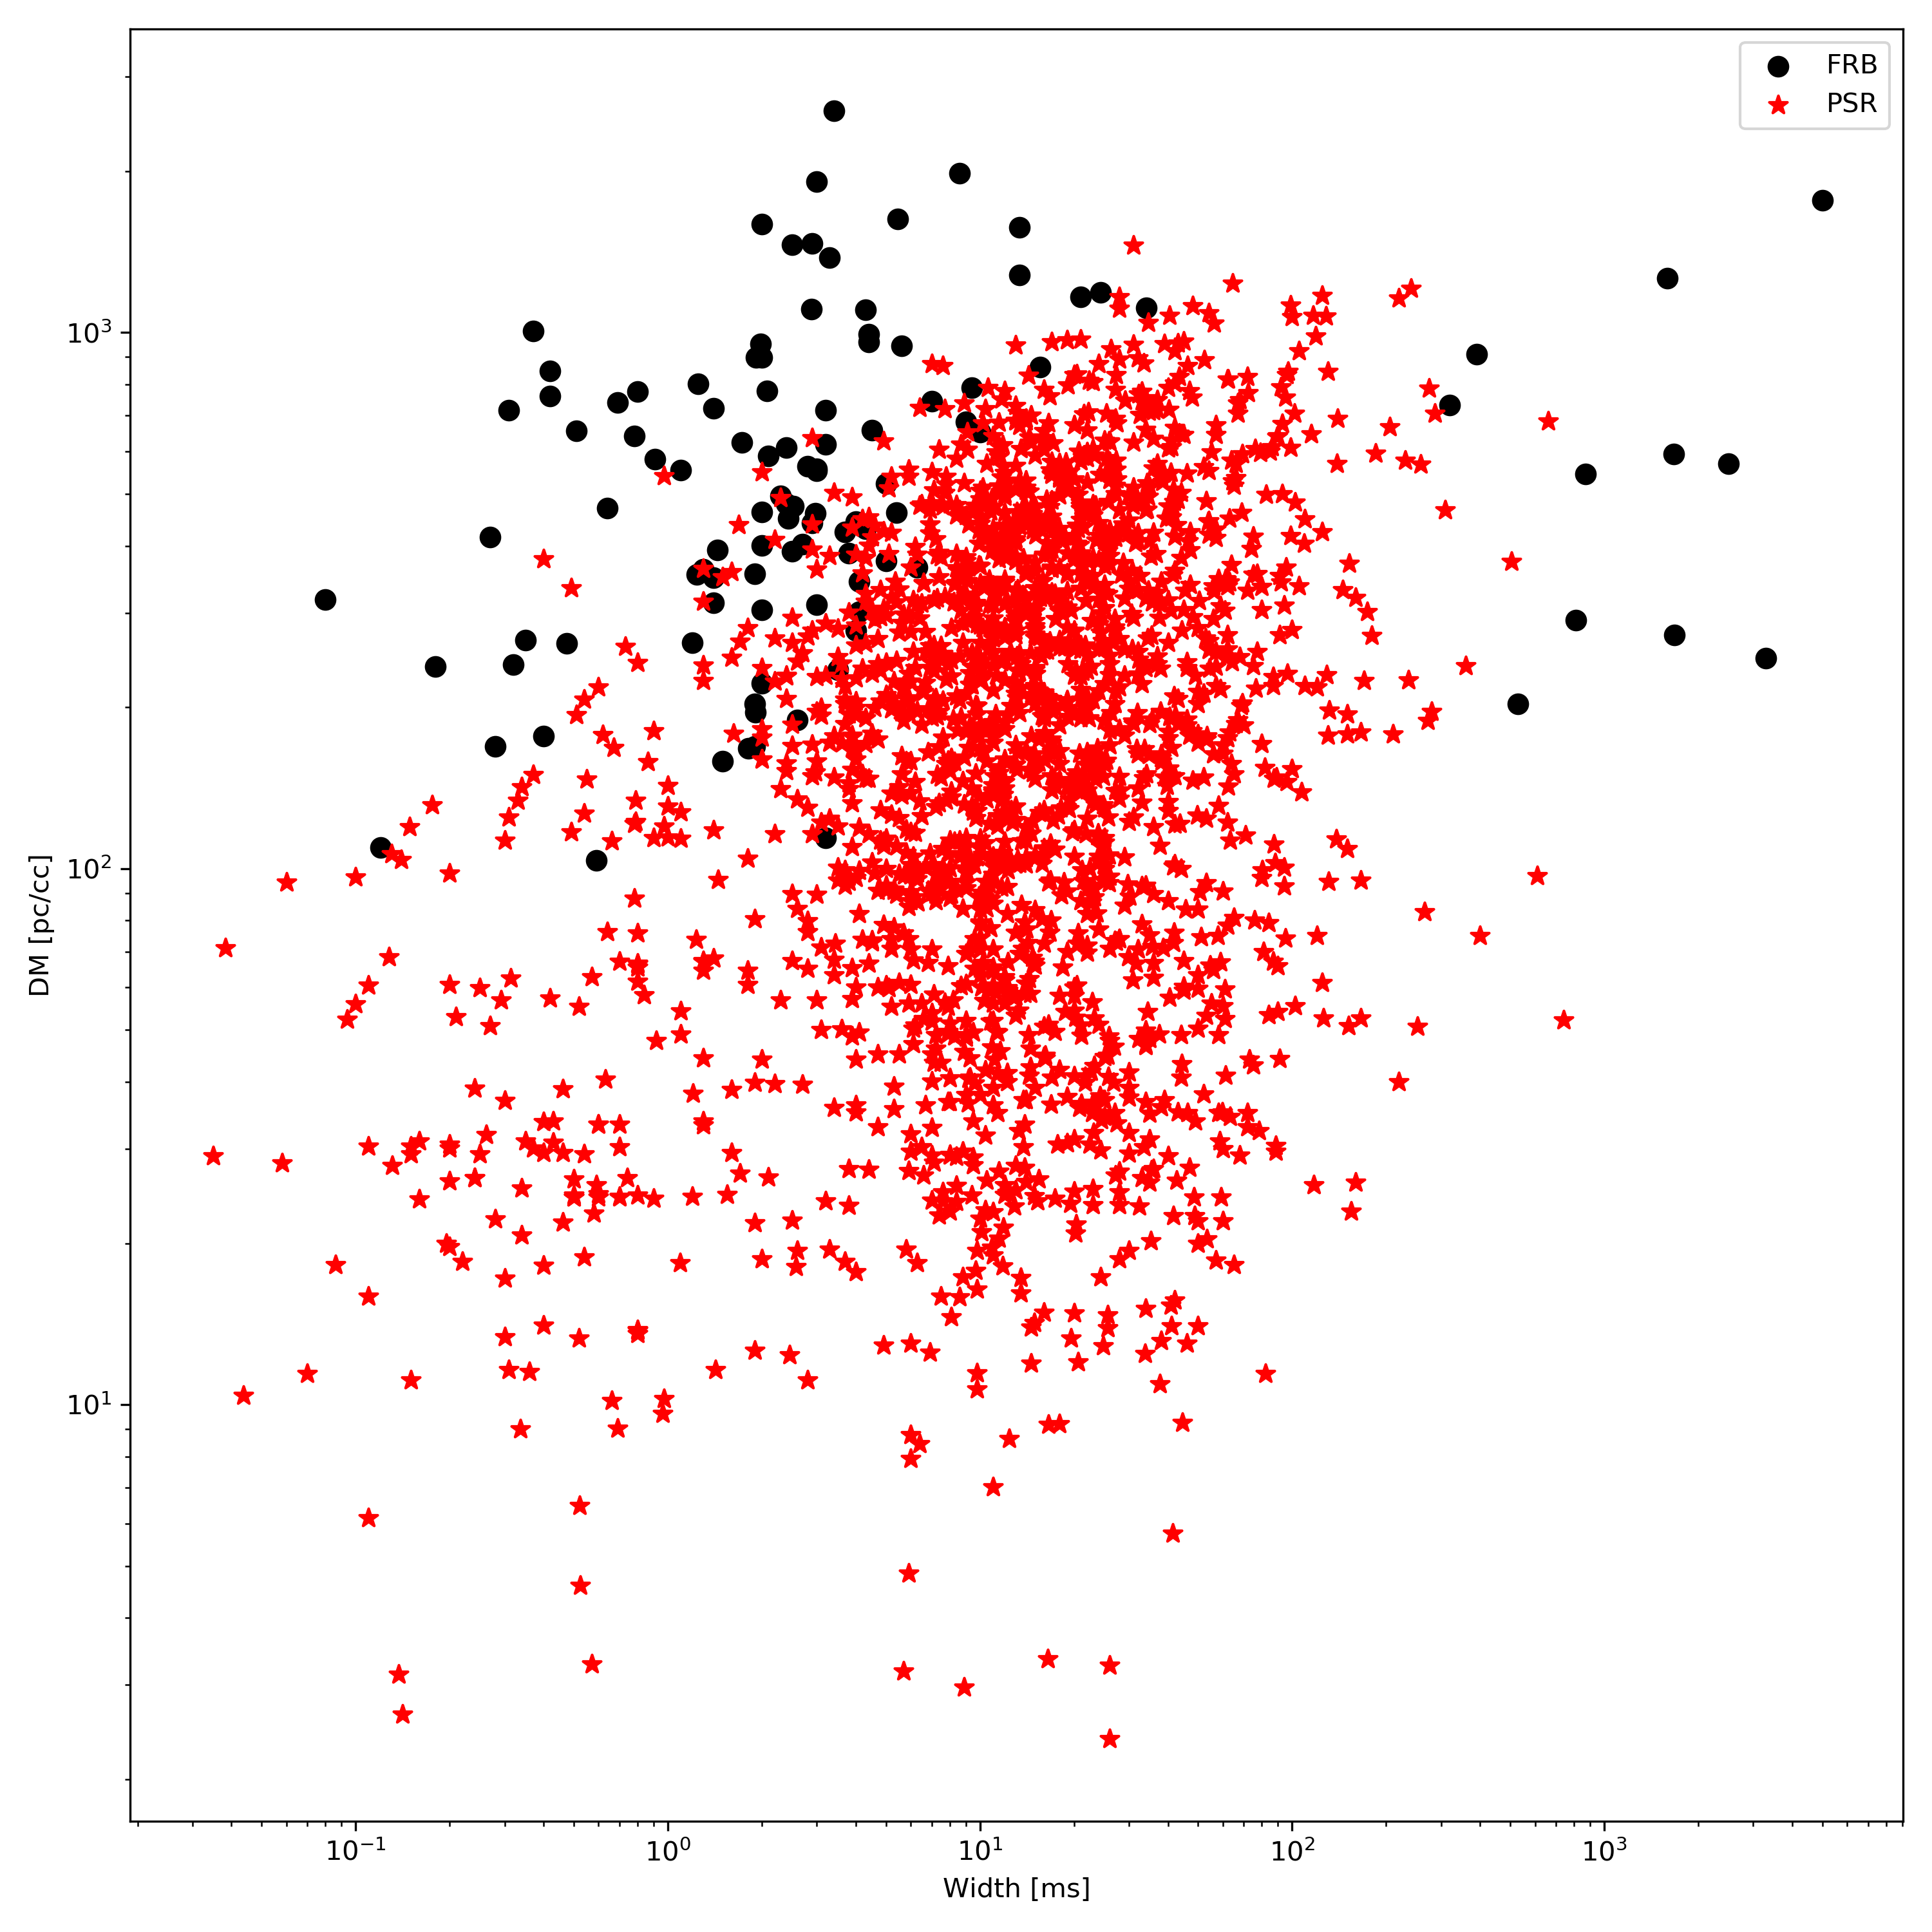
\includegraphics[width=\textwidth,keepaspectratio]{frbpsr_scatter.png}
\label{fig:scatter}
\caption{PSRs and FRBs scatter plot of DM and Width}
\end{figure}
%% higher DM more reach final frontier is pushed further back
\end{frame}

\begin{frame}
\begin{figure}
\centering
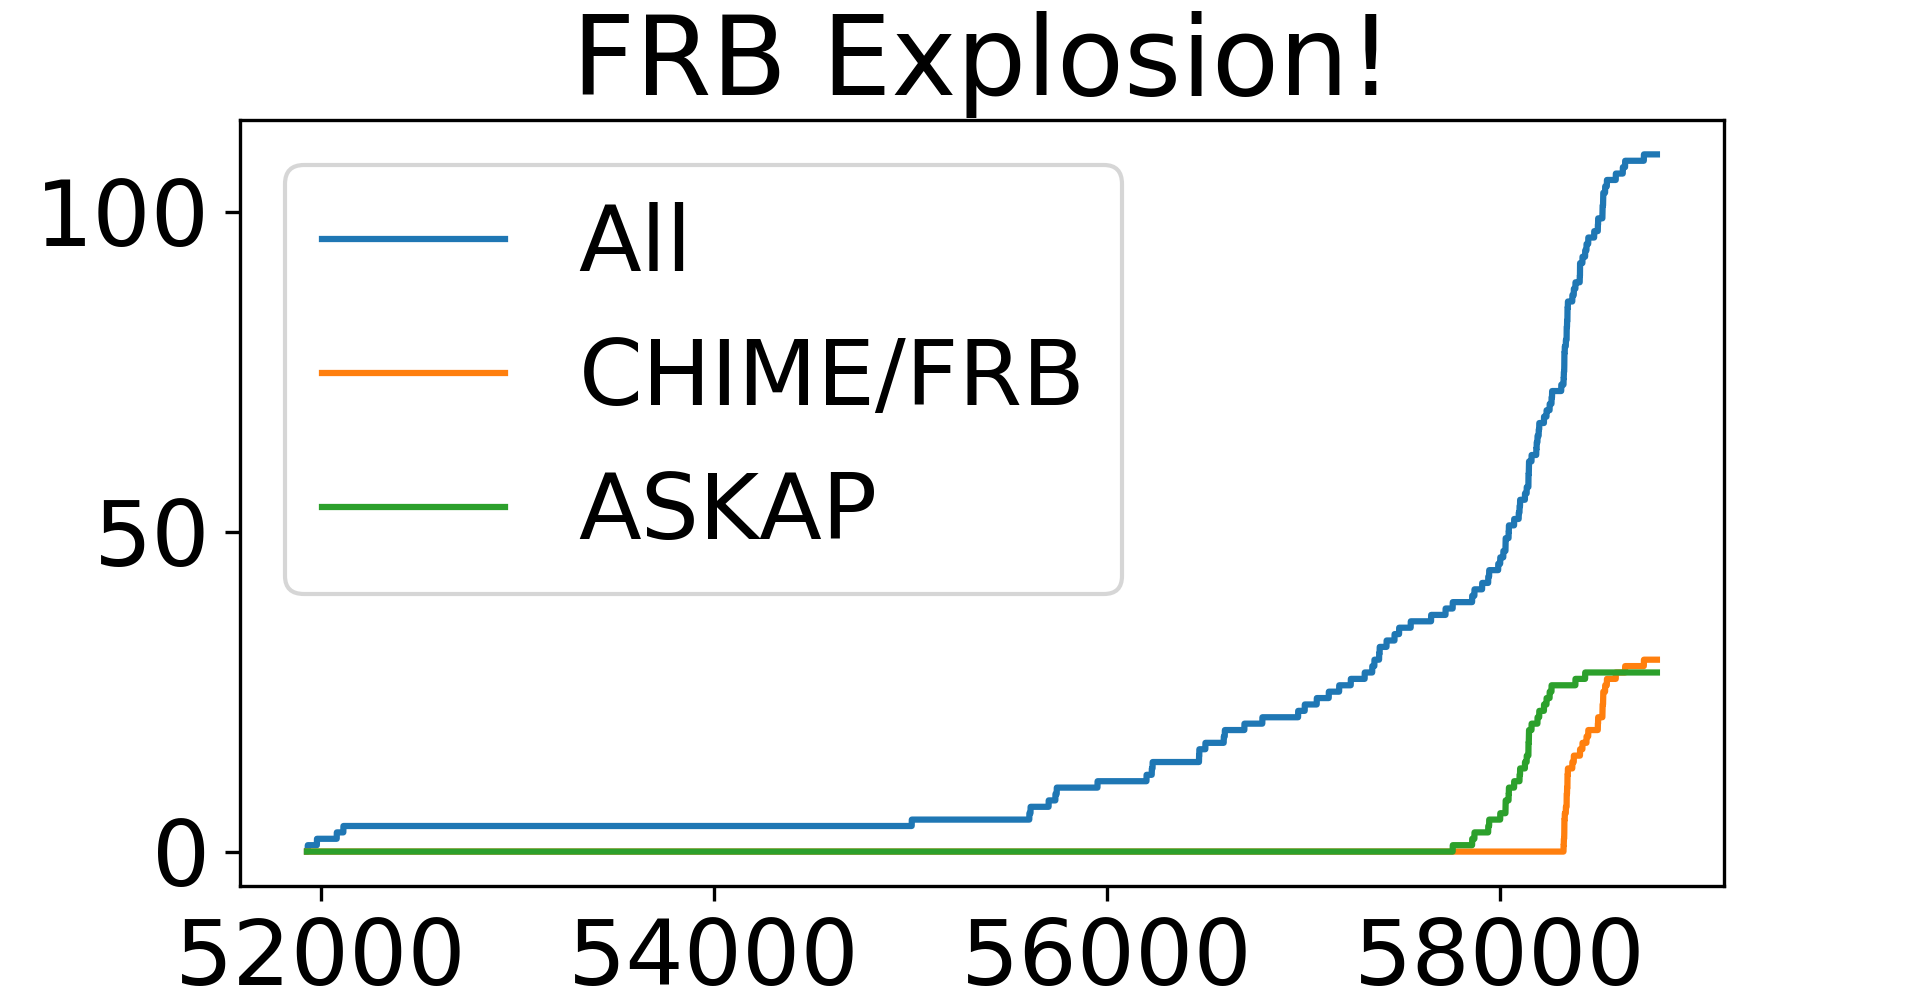
\includegraphics[width=\textwidth,keepaspectratio]{frbexplosion.png}
\label{fig:frbx}
\caption{Cumulative time plot. FRB explosion!}
\end{figure}
%% lot of research effort has already flown in. 
\end{frame}



\section{VLITE-Fast}
\begin{frame}{VLITE-Fast}
\begin{figure}
	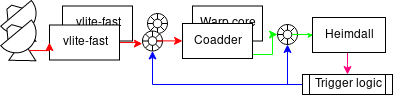
\includegraphics[width=\textwidth,keepaspectratio]{vf_full.png}
\end{figure}
\end{frame}

%% matter tex
%% starts with section in the maintex

\begin{frame}{Single antenna}
\begin{columns}
\begin{column}
	\begin{itemize}
		\item $320|384$ MHz \hfill P-band
		\item 25m dish
		\item Commensal 
		\item Different baselines possible
		\item angular resolution $\sim 0.04\"$
	\end{itemize}
\end{column}
\begin{column}
	\begin{itemize}
		\item vlite-fast codebase developed and maintained by Matthew Kerr
	\end{itemize}
\end{columns}
	\includegraphics[width=\textwidth,keepaspectratio]{single_dish.png}
\end{frame}

\begin{frame}{MPI Coadder \hfill Warp core}
	\begin{itemize}
		\item Incoherent co-addition $\implies$ sensitivity $\sim \sqrt{N_{\rm ant}}$
		\item \emph{One bad apple spoils the bunch} \\
			Median Absolute Deviation (MAD) based time-frequency zapping.
		\item $12$ node GPU-backed Infiniband-connected cluster.
		\item Message Passing Interface tuned for real-time performance.
			\begin{itemize}
				\item \textttt{MCA Collective Reduce = Rabenseifner}
				\item Disable all ethernet (tcp) communications!
				\item \dots
			\end{itemize}
		\item Successfully clocked in days time of operation in one stretch.
	\end{itemize}
\end{frame}

\begin{frame}{Heimdall | GPU program}
	\begin{itemize}
		\item Written by Ben Bardsdell during his PhD at Swinburne!
		\item Matched-filter based approach. 
	\end{itemize}
	\begin{listing}
		for DM in DM-trial
			for Width in 2**[0..MaxWidth] 
				MatchedFilter (Dedisperse(Input, DM), Width)
			end
		end
	\end{listing}
	\begin{itemize}
		\item DM-level coincidencing \hfill Max S/N
		\item Very high False Positive rates!
	\end{itemize}
\end{frame}

\begin{frame}{Triggering logic | End products}
	\begin{itemize}
		\item Currently applying cuts: 
		\begin{align}
			{\rm S/N} &\geq 8.5 \\
			{\rm DM}  &\geq 50 {\rm pc/cc} \\
			{\rm Width} &\geq 10 {\rm ms}
		\end{align}
		\item Two mutually exclusive trigger channels: 
			\begin{itemize}
				\item Filterbank triggering. \hfill \emph{above cuts}
				\item Voltage triggering. \hfill S/N $\geq 25$
			\end{itemize}
		\item End products
			\begin{description}
				\item[Filterbank Triggering] \\ 
					Binary JSON file. \\
					Filterbank data.
				\item[Voltage Triggering] \\
					Raw binary file dump. \\
					Two polarization voltage series.
			\end{description}
		\item An $8$-second of voltage data is $\sim 48$x more space than filterbank data.
	\end{itemize}
\end{frame}

\begin{frame}{Codebases}
\begin{columns}
	\begin{column}
	\begin{itemize}
		\item \textbf{\large Asgard} \hfill C++11
		\item MPI Coadder
		\item Filterbank triggering
		\item Regular data analysis, visualization, and meta analysis.
	\end{itemize}
	\end{column}

	\begin{column}
	\begin{itemize}
		\item \textbf{\large vlite-fast} \hfill C,CUDA
		\item Maintained and developed by \textbf{ Matthew Kerr } \emph{ (co-advisor) }
		\item Voltage packets from antennas $\to$ filterbanking on GPU
	\end{itemize}
	\end{column}
\end{columns}
\end{frame}


\section{Searches}
%% matter tex
%% starts with section in the maintex

\subsection {NBITS=2}
\begin{frame}{00,01,10,11}
\begin{itemize}
	\item In an epoch from \hfill 2019-10-17 23:15:11
	\item to \hfill 2019-12-05 13:43:19
	\item with onsky time \hfill 27 days, 1:05:24
	\item with offsky time \hfill 21 days, 13:22:44
	\item achieving uptime \hfill $55.65\%$
	\item recording \hfill $10573$ fbsons
	\item trigger rate \hfill $13/{\rm hr}$
	\item with minimum antennas \hfill $12$
	\item FRBs: \hfill \textbf{\Large 0}
\end{itemize}
\end{frame}

\subsection {NBITS=8}
\begin{frame}{0x00..0xFF}
\begin{itemize}
	\item In an epoch from          \hfill 2019-12-10 23:13:23
	\item to                        \hfill 2020-01-20 21:04:16 
	\item with onsky time           \hfill 16 days, 15:34:12 
	\item with offsky time          \hfill 24 days, 6:16:41
	\item achieving uptime          \hfill $40.70\%$
	\item recording                 \hfill $4950$ fbsons
	\item trigger rate              \hfill $\sim 13/{\rm hr}$
	\item with minimum antennas     \hfill $13$
	\item FRBs:                     \hfill \textbf{\Large 0}
\end{itemize}
\end{frame}

\subsection {Coaddition effects}
\begin{frame}{Power of coaddition}

\begin{columns}[onlytextwidth]
\column{0.7\textwidth}
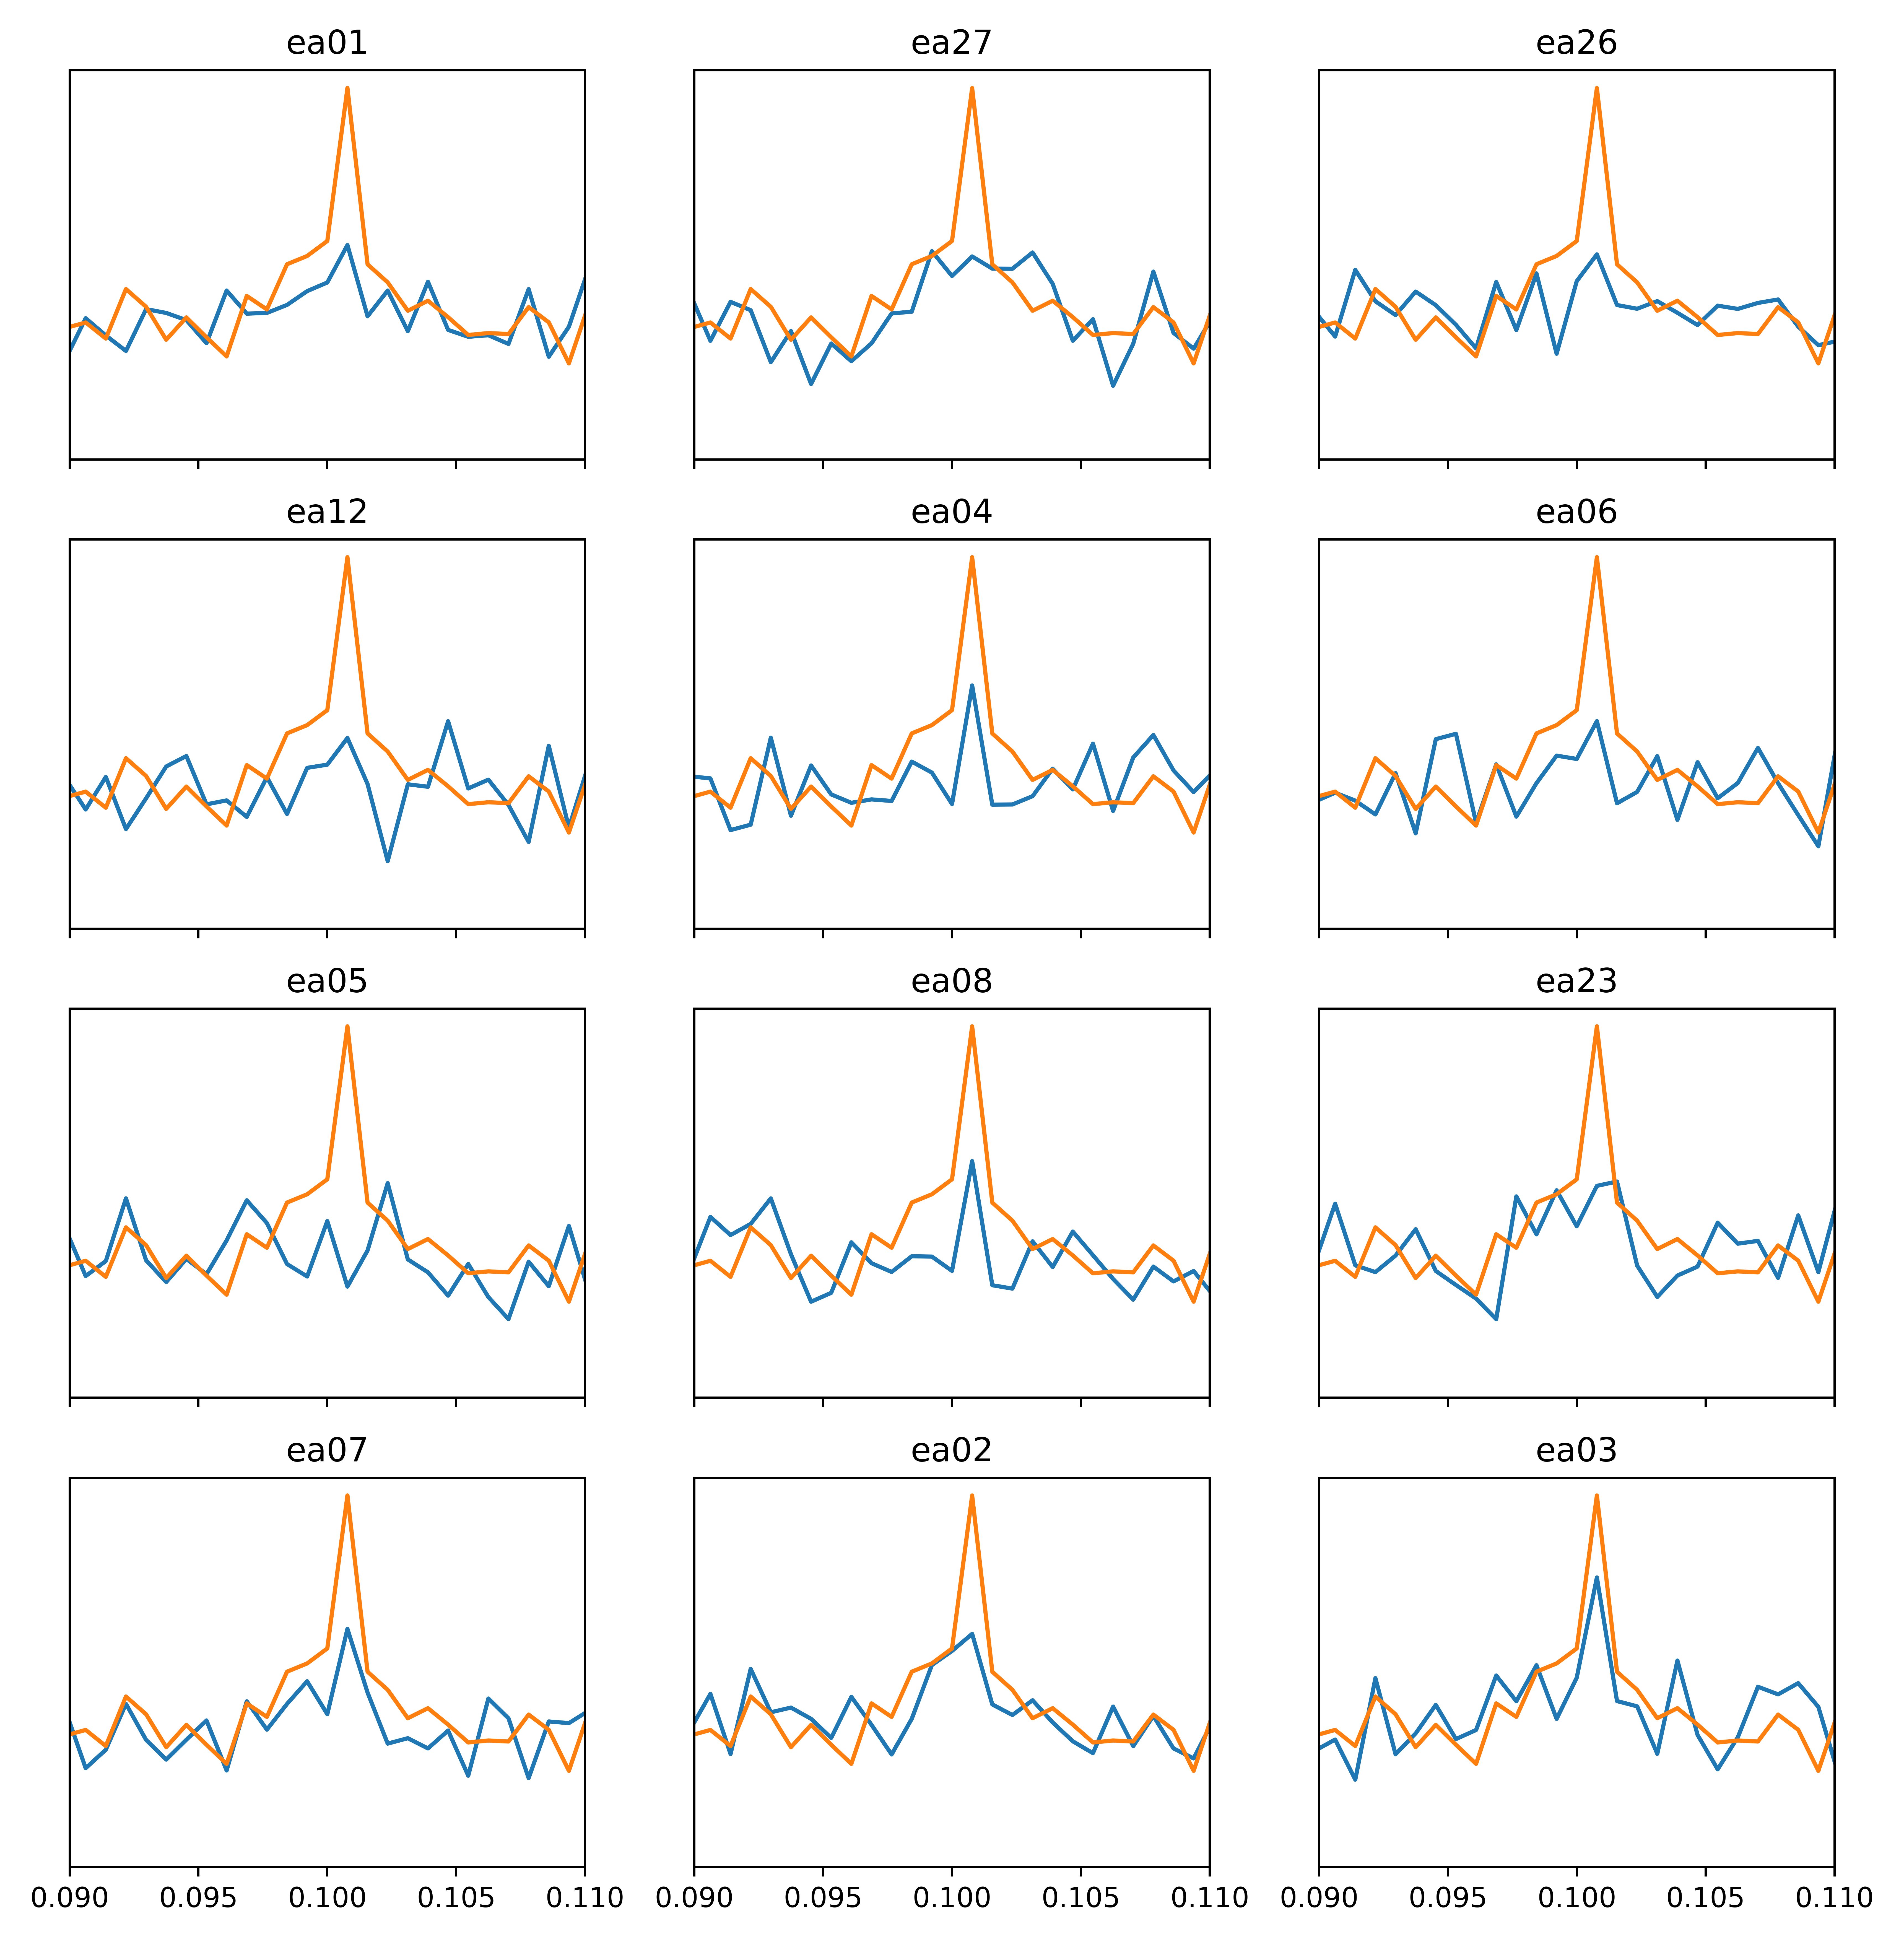
\includegraphics[width=\textwidth,keepaspectratio]{psr_low_4x3.png}
\column{0.3\textwidth}
\begin{itemize}
    \item Orange is coadded. 
    \item Noise suppresion and signal enhancement.
\end{itemize}
\end{columns}
\end{frame}

\begin{frame}{Pulses from Pulsars!}
	\begin{figure}
		\centering
		\includegraphics[width=0.8\textwidth,keepaspectratio]{radec_psr.png}
		\label{fig:fov}
		\caption{PSR\,J0534$+$2200, \textcolor{green}{(green star)}, PSR\,J1752$-$2806 \textcolor{red}{( transparent red star )}}
	\end{figure}
\end{frame}


\section{Thesis}
%% actual thesis slides


\begin{frame}
\begin{center}
\vspace*{\vfill}
\texttt{\large Thesis title:}\\
\texttt{\Huge Increasing sensitivity to FRBs through ML}
\vspace*{\vfill}
\end{center}
\end{frame}

\begin{frame}{Why?}
\begin{itemize}
		\item Currently applying cuts: 
		\begin{align}
			{\rm S/N} &\geq 8.5 \\
			{\rm DM}  &\geq 50 {\rm pc/cc} \\
			{\rm Width} &\leq 100 {\rm ms}
		\end{align} $\implies$ trigger-rate $\approx 13/$hr.
		\item Reducing S/N would significantly increase the trigger rate.
		\item False positives waste: \begin{itemize}
			\item Disk space on SSD
			\item CPU, human time
			\item Strain on triggering system
				%% system could have worked on other trigger
		\end{itemize}
	\item Machine Learning (ML) as next step in searching.
\end{itemize}
\end{frame}

\begin{frame}{How?}
\begin{itemize}
	\item Input  := Dispersed filterbank chuck
	\item Output := Decision
	\item Required constraints: 
		\begin{description}
		\item[Fast] Realtime capability
		\item[Throughput] Handle Radio Frequency Interference (RFI) strikes
		\item[$\leq$Moderate-weight] Not be computationally demanding
		\end{description}
	\item \emph{A fast ML solution capable of running realtime.}
\end{itemize}
\end{frame}

\subsection{Feature engineering}
\begin{frame}{Bowtie plane}
\begin{columns}[onlytextwidth]
\column{0.7\textwidth}
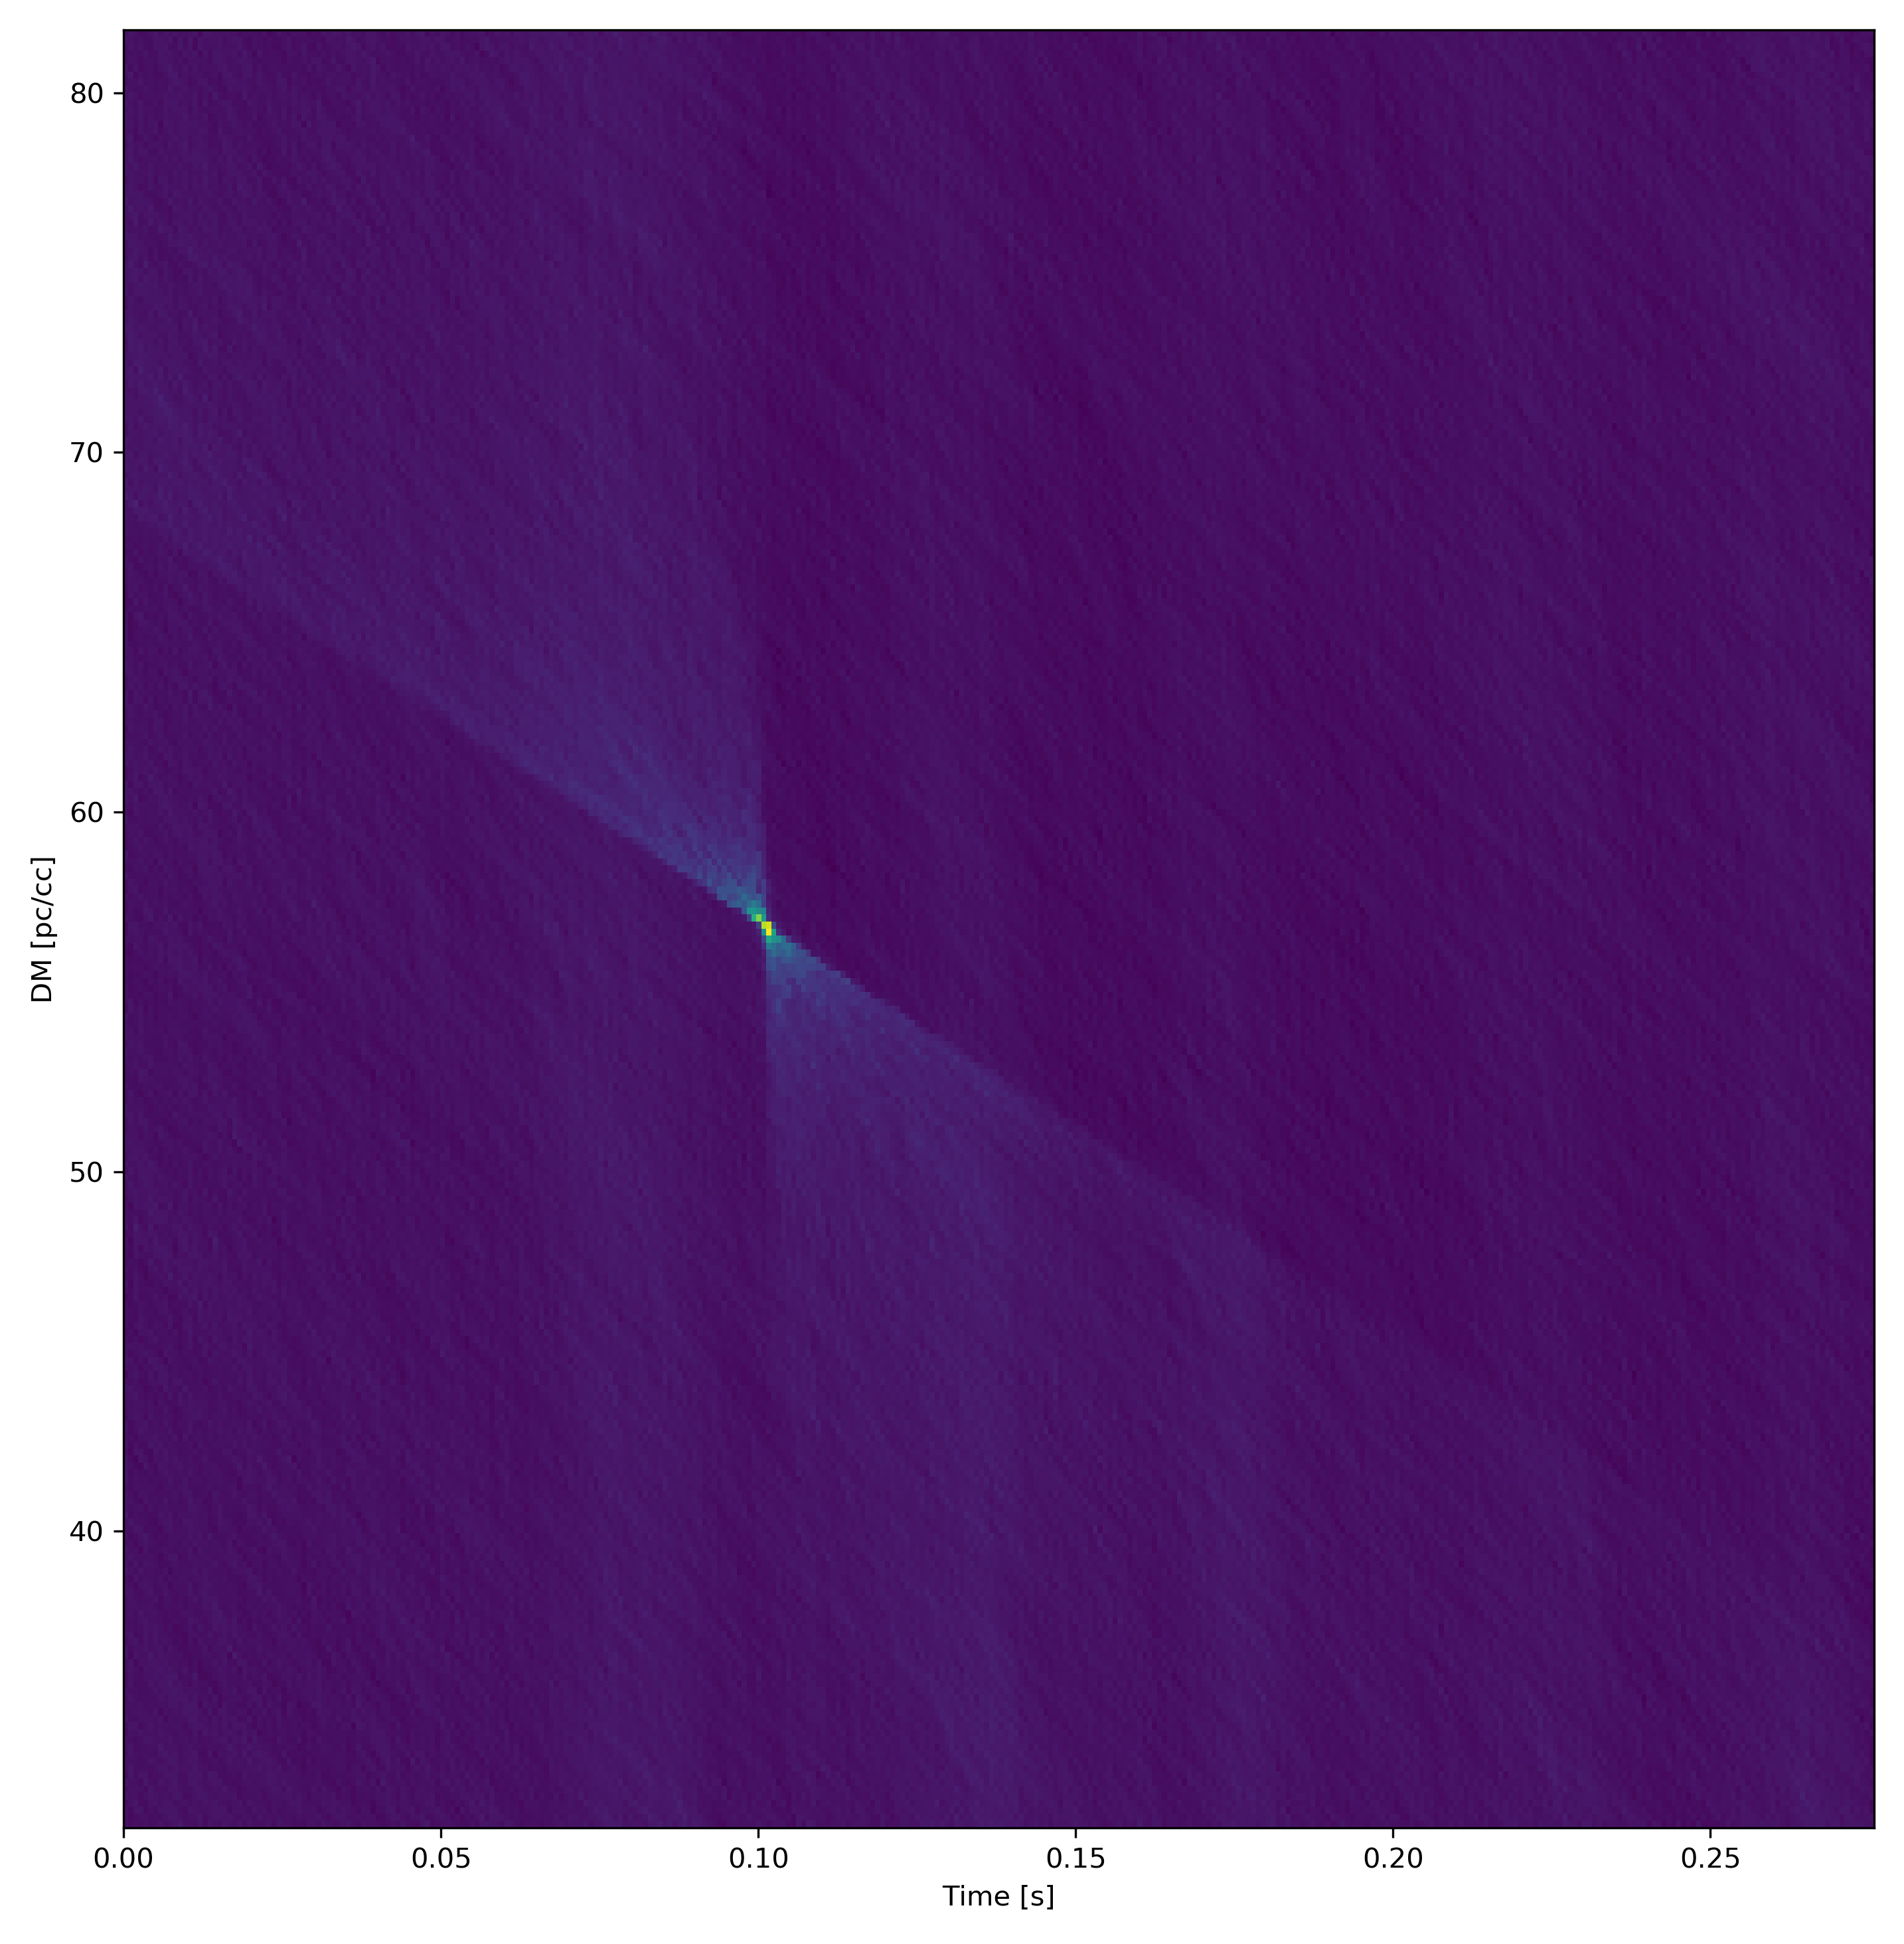
\includegraphics[width=\textwidth,keepaspectratio]{bt_flat.png}
\column{0.3\textwidth}
\begin{itemize}
    \item Offsource ping from Crab psr. S/N=106.58 \emph{(highest)}
\end{itemize}
\end{columns}
\end{frame}

\begin{frame}
	\begin{figure}
	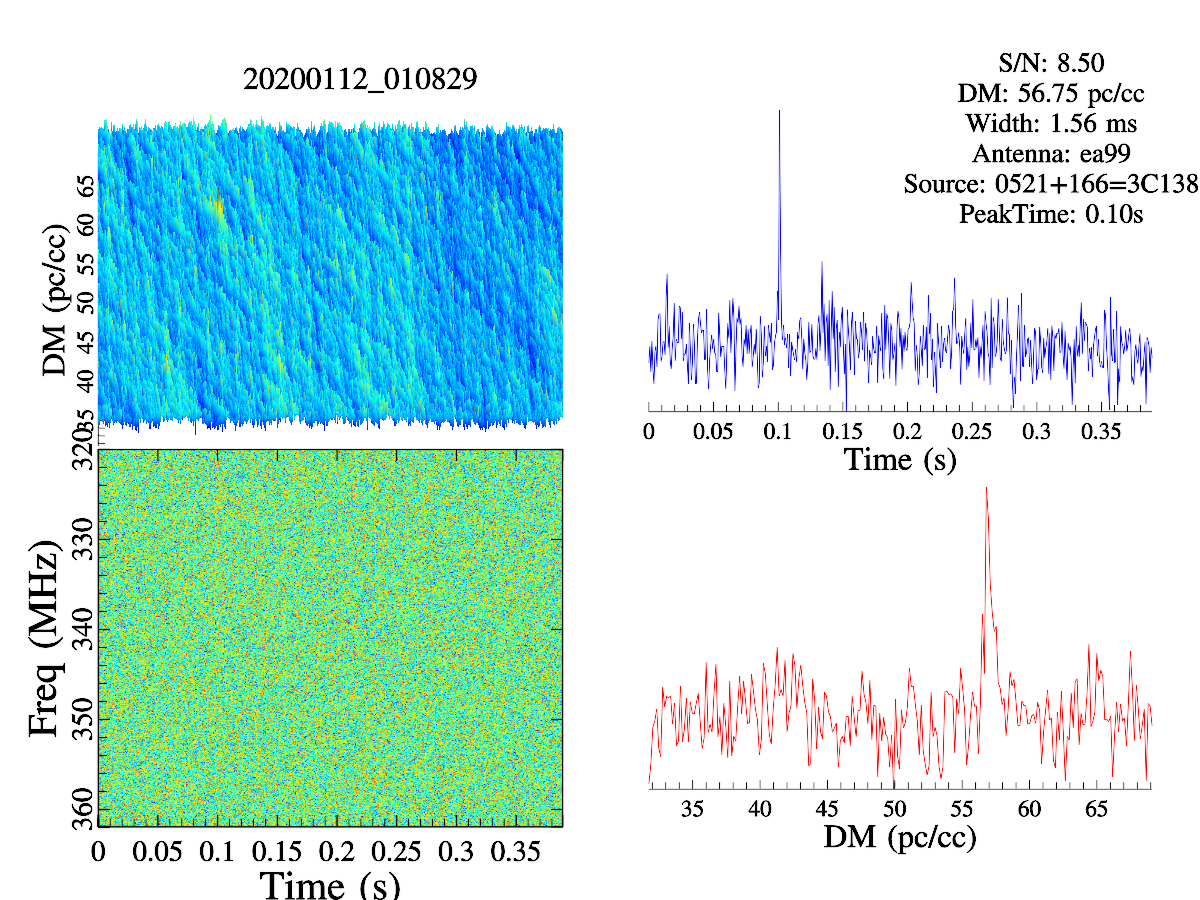
\includegraphics[width=\textwidth,keepaspectratio]{candplot.png}
	\label{fig:candplot}
	\end{figure}
\end{frame}

\begin{frame}[allowframebreaks]{Featureset | Lyon features~\cite{lyon}}
\begin{itemize}
	\item First four standardized moments (mean, variance, skewness, and kurtosis) of \begin{itemize}
			\item S/N as a function of time
			\item S/N as a function of DM
		\end{itemize}
	\item $\mathcal{O}(N)$ operation
	\item Bowtie plane: the most computationally expensive.
	\item Fast De-dispersion Measure Transform (FDMT) \hfill \cite{fdmt}
\end{itemize}
\end{frame}

\begin{frame}{Power of skewness and kurtosis}
\begin{columns}[onlytextwidth]
\column{0.7\textwidth}
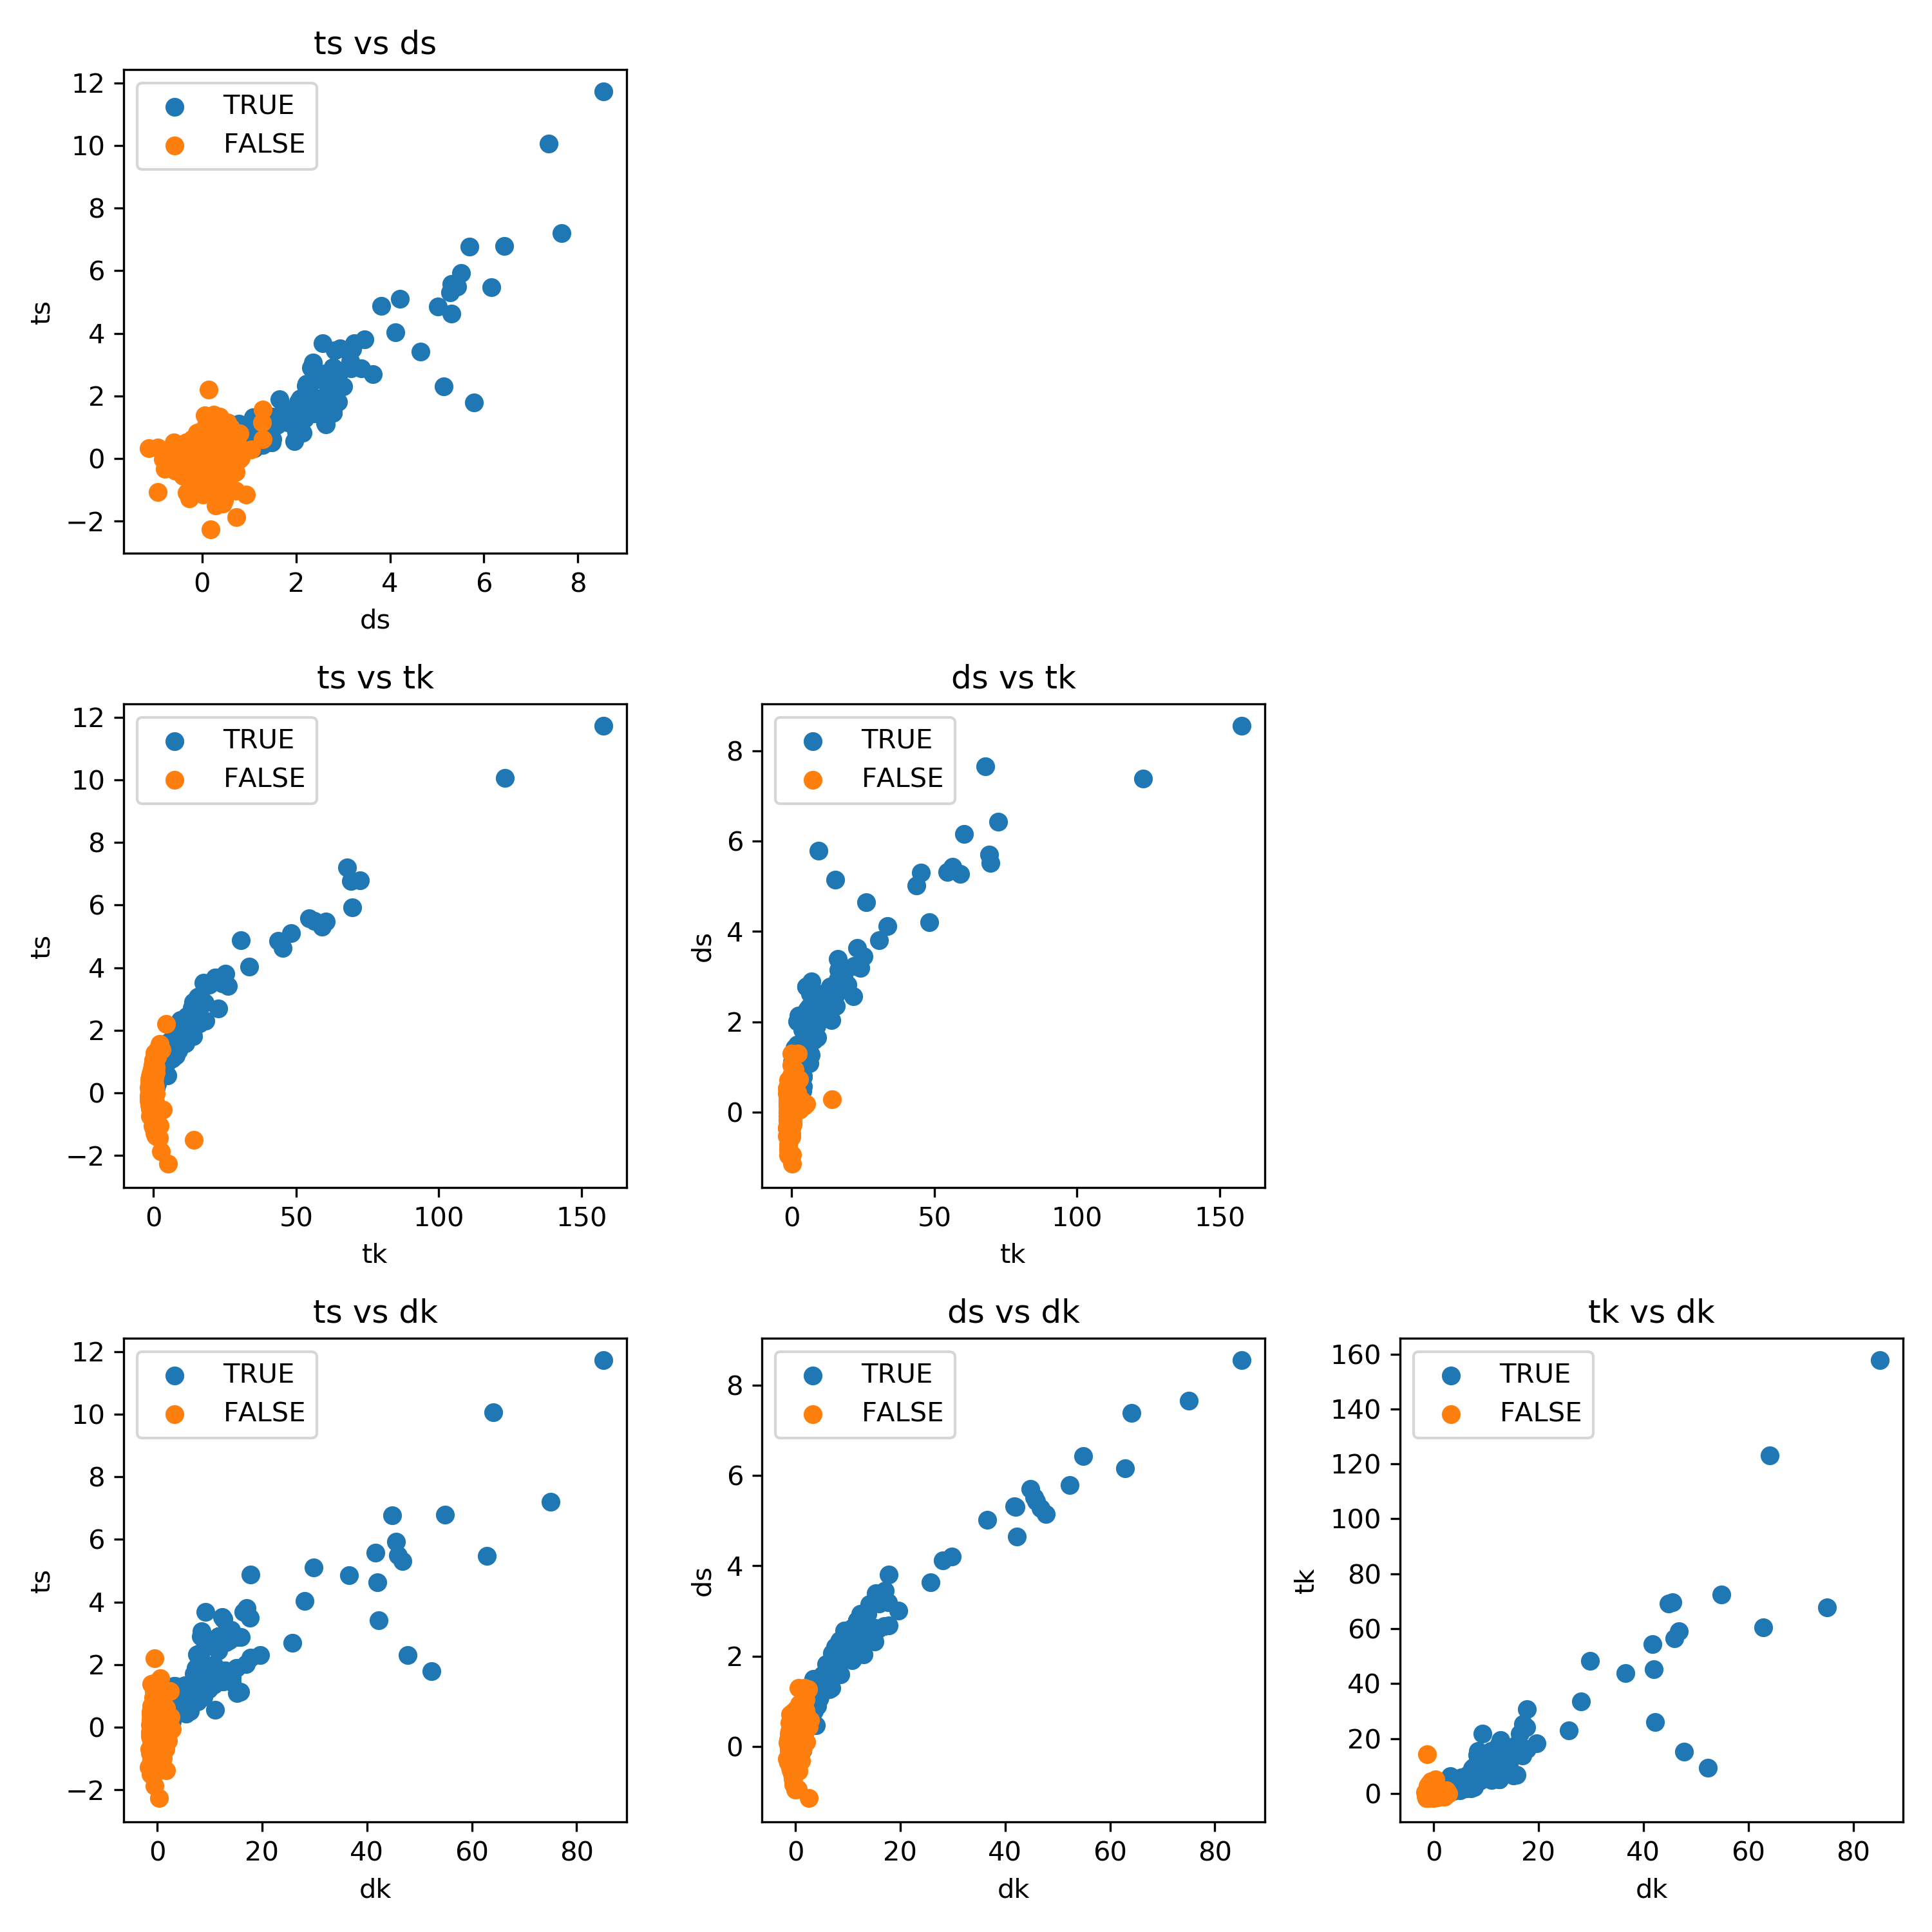
\includegraphics[width=\textwidth,keepaspectratio]{corner_td_sk.png}
\column{0.3\textwidth}
\begin{itemize}
    \item Not linearly separable! But some structure for ML!
    \item Tree based ML
    \item Support Vector Machine with kernel trick
    \item Discriminability. Skewness and kurtosis of S/N(t),S/N(DM).
\end{itemize}
\end{columns}
\end{frame}

\begin{frame}
\vspace{\vfill}
{\Huge Still a long way!}
\vspace{\vfill}
\end{frame}


\section{Trishul}
%% matter

\begin{frame}{Trishul}
\begin{itemize}
	\item Trishul, Sanskrit for Trident
	\item One weapon for dispersed transient searches:
		\begin{itemize}
			\item Searching \hfill On bowtie plane
			\item Vetting   \hfill Machine Learning
			\item Dumping/Plotting \hfill JSON, MathGL
		\end{itemize}
	\item C++ $\sim 3k$ loc
	\item Reusing pieces! \hfill Polishing them!
	\item \emph{Very ambitious version of my thesis!}
\end{itemize}
\vspace{\vfill}
{\Huge The End!}
\vspace{\vfill}
\end{frame}


\end{document}
